
\label{ch:tests}

Test cases for CISM include experiments with analytic solutions, standardized experiments
without analytic solutions but for which community benchmarks are available, and
some experiments specific to CISM which have been well characterized by CISM developers.

Here we organize test cases based on the velocity solver that is most appropriate
for each test.  Any velocity solver can be used with any test
if the .config file settings are adjusted manually.  In some cases, however, the results
may be difficult to interpret.

Each test directory includes a README file with some technical details 
about how to run the test.  Many tests have python scripts that are used to set up
the initial condition and, in some cases, execute the model.  Some tests
have an additional python script for analyzing the CISM output.

The user must manually provide each test with access to the CISM executable.
There are several ways to do this:

\begin{itemize}
  \item Softlink the executable into the directory, e.g.:

        \texttt{ln -s ../../../builds/mac-gnu/cism\_driver/cism\_driver ./}

        This is the recommended procedure during development so that the test
        will always be using the most up-to-date version of the executable.

  \item Use the -e command line option to point to include an explicit path for the executable (for test case run scripts that support this option), e.g.:

        \texttt{./dome.py -e ../../../builds/mac-gnu/cism\_driver/cism\_driver}

        This is useful for quickly trying a different version of CISM (e.g., comparing 
        serial and parallel executables).

  \item Add the directory containing the CISM executable to your environment PATH.

  \item Copy the executable into the directory.  This is typically not the most efficient approach,
        but may make sense in some situations.
\end{itemize}

The python scripts generally have useful
command line options that control their execution.  Typically, you can see details 
by using the \texttt{-{}-help} (or \texttt{-h}) command line option, e.g.:

\texttt{./dome.py --help}

The various tests are described below.

% =====================================

\section{Shallow Ice Test Cases}
\label{sc:sia-tests}

These tests are primarily useful for testing the shallow-ice approximation (SIA) dynanmical core (Glide; see Chapter \ref{ch:glide}).

% =====================================
\subsection{Halfar dome}
% =====================================

\label{sec:halfar_description}
This test case describes the time evolution of a parabolic-shaped dome of ice, as described by \citet{Halfar1983}.
For a flat-bedded SIA problem, this test case has an analytic solution for the time varying ice thickness. We start with the
general SIA ice evolution equation,  

\begin{equation}
    \label{halfar}
    \frac{\partial H}{\partial t} = \nabla \cdot (\Gamma H^{n+2} |\nabla H|^{n-1} \nabla H),
\end{equation}

where $n$ is the exponent in the Glen flow law, commonly taken as 3, and $\Gamma$ is a positive constant:

\begin{equation}
    \Gamma = \frac{2}{n+2} A (\rho g)^n.
\end{equation}

For $n=3$, this reduces to:

\begin{equation}
    H(t,r) = H_0 \left(\frac{t_0}{t}\right)^\frac{1}{9}  \left[ 1 - \left(  \left( \frac{t_0}{t} \right) ^ \frac{1}{18} \frac{r}{R_0} \right)^\frac{4}{3} \right] ^ \frac{3}{7},
\end{equation}

where

\begin{equation}
    t_0 = \frac{1}{18\Gamma} \left( \frac{7}{4} \right)^3 \frac{R_0^4}{H_0^7},
\end{equation}

and $H_0, R_0$ are the central height of the dome and its radius at time $t=t_0$.

For more details see \citet{Halfar1983}, \citet{Bueler2005}, and this \href{http://www.projects.science.uu.nl/iceclimate/karthaus/2009/more/lecturenotes/EdBueler.pdf}{link}\footnote{http://www.projects.science.uu.nl/iceclimate/karthaus/2009/more/lecturenotes/EdBueler.pdf}.

\subsubsection{Provided Files}
\label{subsec:halfar_files}

Our implementation of the Halfar dome test has an initial radius of $R_0=21.2$ km and an initial thickness of $H=707.1$ m.
These values can be changed by editing \texttt{halfarDome.py}.

\begin{itemize}
	\item README \\
		Information about the test case, including technical details about running it.
	\item halfar.config \\
		This is the config file defining CISM options. \\
              The version \texttt{halfarHO.config} is setup to run using the GLISSADE dycore.
	\item halfar.py \\
		This python script generates the dome initial condition and runs CISM.
	\item halfar\_results.py \\
		This is script compares model results to the analytic solution.
	\item halfarDome.py \\
		This is a python module that defines the analytic solution. \\
    		 It is not meant to be run manually, but it is used by the other scripts.
\end{itemize}

\subsubsection{Running the test}
One script sets up the initial condition and runs the model:

\texttt{./halfar.py}

Another script analyzes the results:

\texttt{halfar\_results.py}

\subsubsection{Results}
\label{subsecc:halfar_results}
With the default .config settings, this simulation should only take a few seconds and is a good first test for a working GLIDE dycore.
As the dome of ice evolves, its margin advances and its thickness decreases (there is no surface mass balance to add new mass).  The script \texttt{halfar\_results.py} will plot the modeled and analytic thickness at a specified time (Figure \ref{fig:halfarresults}), as well as report model error statistics.  Invoke \texttt{halfar\_results.py --help} for details on its usage.


\begin{figure}[H]
	\centering
	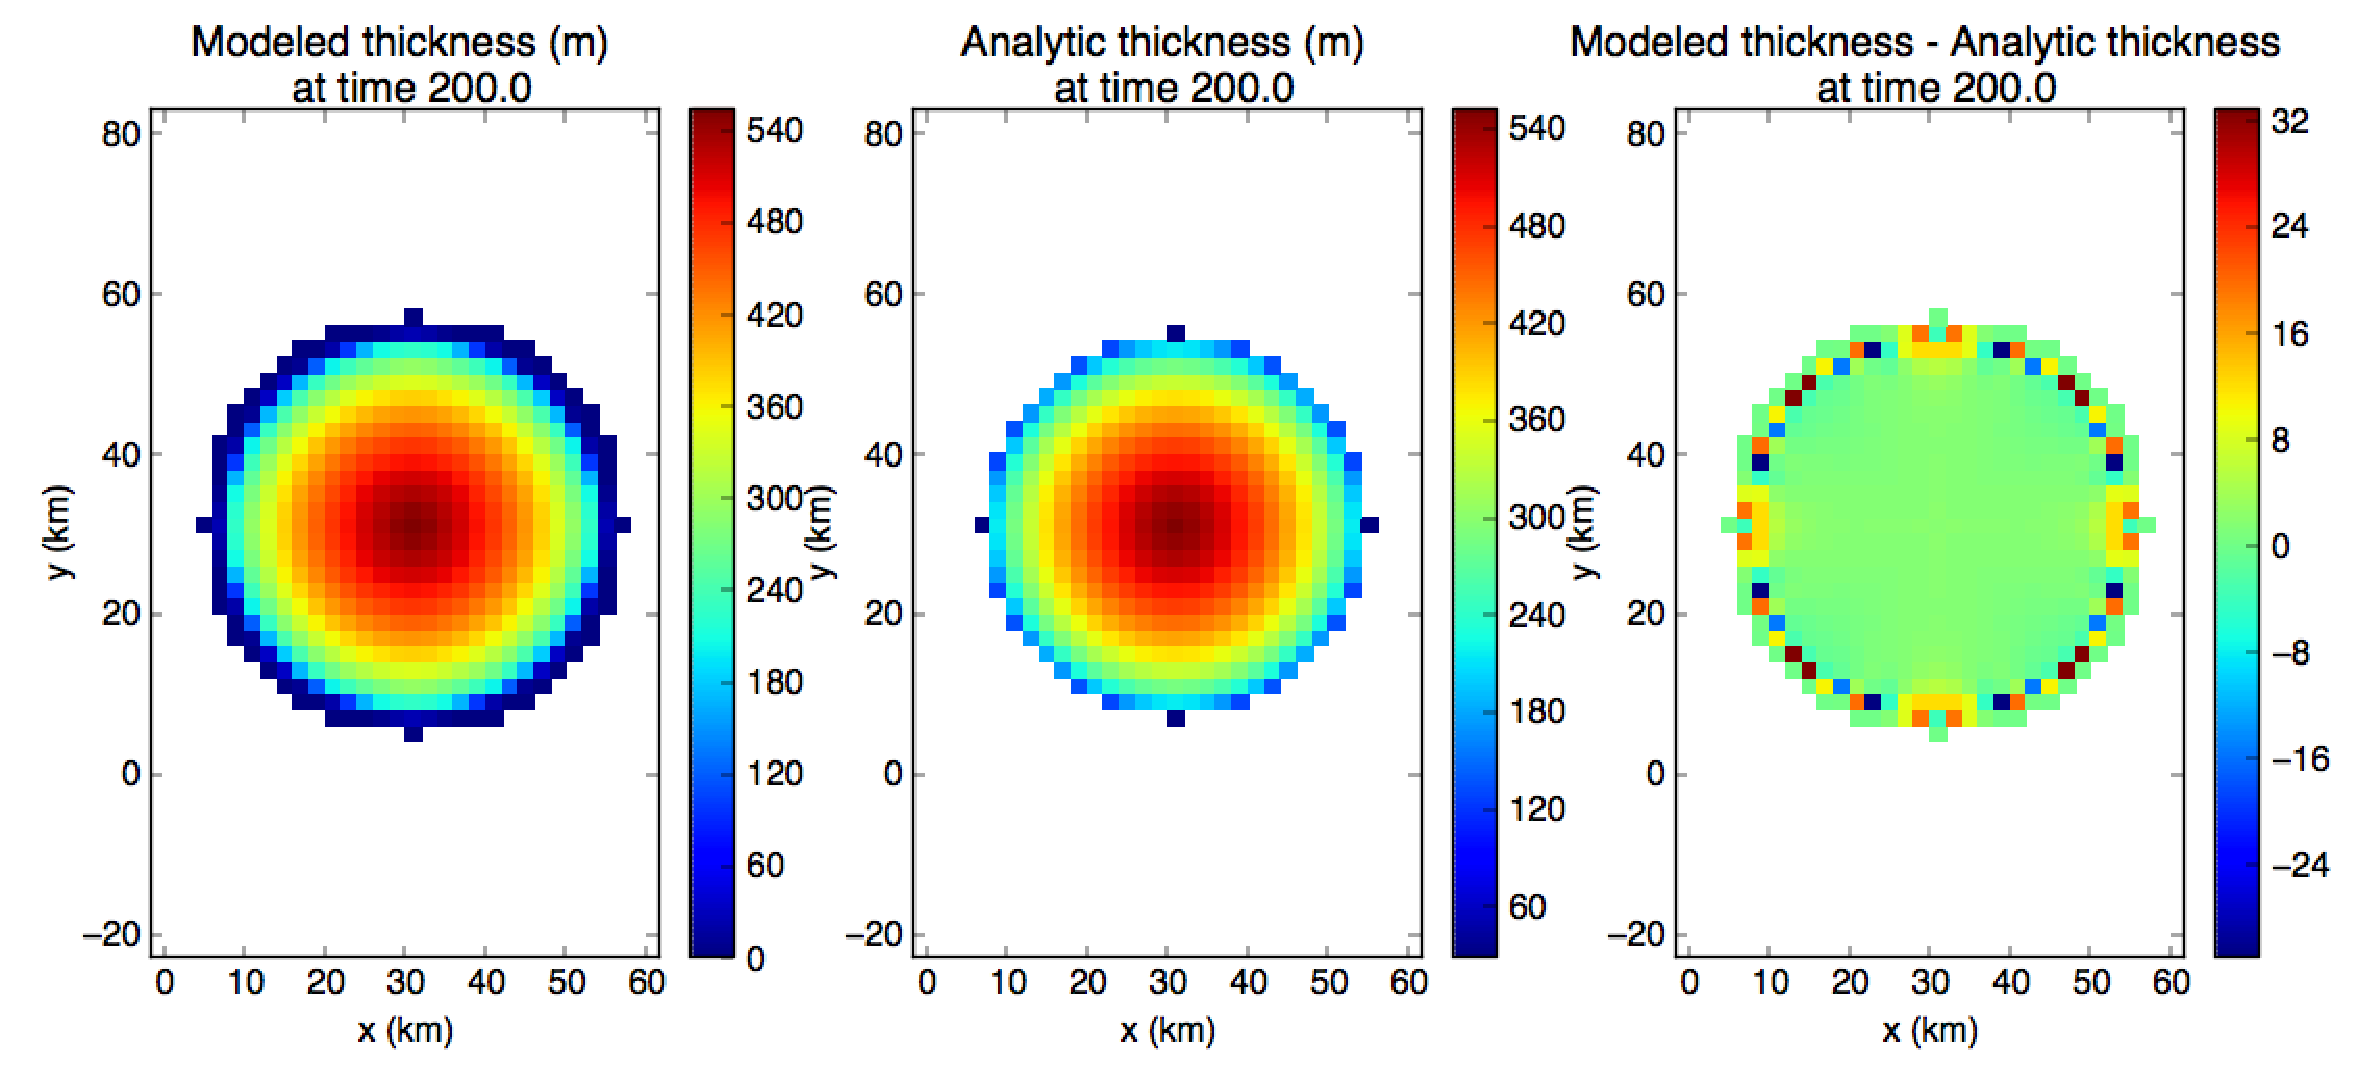
\includegraphics[width=16.4cm]{\dir/halfar_results.eps}
	\caption{Halfar test case results after 200 years of dome evolution. This figure is generated by \texttt{halfar\_results.py}.}
	\label{fig:halfarresults}
\end{figure}


\FloatBarrier


% =====================================
\subsection{EISMINT-1}
% =====================================
\label{sec:eismint_description}
This test case is from phase 1 of the European Ice Sheet Modelling INiTiative intercomparison experiments.  These experiments are described in more detail
\href{http://homepages.vub.ac.be/~phuybrec/eismint.html}{here}\footnote{http://homepages.vub.ac.be/~phuybrec/eismint.html} and in \citet{Huybrechts1996}.

\subsubsection{Provided Files}
\label{subsec:eismint_files}

\begin{itemize}
	\item README \\
	Information about the test case, including technical details about running it.
	\item *.config \\
  	There are six .config files for each of the six experiments in EISMINT 1.  There are three fixed margin experiments (fm) and three moving margin experiments (mm).
\end{itemize}

\subsubsection{Running the test}
There is not a script for running these experiments, they are simply run manually, e.g. using: 

\texttt{./cism\_driver e1-fm.1.config}

\subsubsection{Results}
\label{subsecc:eismint_results}
These experiments are meant to be run to steady-state, and the supplied .config files are setup to run for long enough for it to be reached.
These simulations take more than a few minutes to complete.
As the initial ice sheet evolves, its shape eventually reaches a steady-state with the imposed surface mass balance.  Currently there is not a script for analyzing the CISM results.  However, users can visually compare their results to those in the \citet{Huybrechts1996} paper.


% =====================================
\subsection{EISMINT-2}
% =====================================
\label{sec:eismint2_description}
This test case is from phase 2 of the European Ice Sheet Modelling INiTiative intercomparison experiments.  These experiments are described in more detail
\href{http://homepages.vub.ac.be/~phuybrec/eismint.html}{here}\footnote{http://homepages.vub.ac.be/~phuybrec/eismint.html} and in \citet{Payne2000}.

\subsubsection{Provided Files}
\label{subsec:eismint2_files}

\begin{itemize}
	\item README \\
	Information about the test case, including technical details about running it.
  	\item *.config \\
  	There are 11 .config files for each of the a-f experiments in EISMINT-2.
  	\item mound.nc, trough.nc \\
    	These are input netCDF files used by the EISMINT-2 experiments.
\end{itemize}

\subsubsection{Running the test}
There is not a script for running these experiments, they are simply run manually, e.g. using: 

\texttt{./cism\_driver e2.a.config}


\subsubsection{Results}
\label{subsecc:eismint2_results}
These experiments are meant to be run to steady-state, and the supplied .config files are setup to run for long enough for it to be reached.  
Note that some of the experiments use the final state of a previous experiment 
as the initial condition (e.g., most experiments following experiment A use the final steady-state from A as an initial condition).  
See the experimental descriptions in \citet{Payne2000} for details.
These simulations take more than a few minutes to complete.
As the initial ice sheet evolves, its shape eventually reaches a steady-state with the imposed surface mass balance.  Currently there is not a script for analyzing the CISM results.  However, users can visually compare their results to those in the \citet{Payne2000} paper.


% =====================================
\subsection{GLINT example}
% =====================================
\label{sec:glint_example}

\textbf{ *** Glint example description needed here; additional details needed below *** }

\subsubsection{Provided Files}

\begin{itemize}
	\item README \\
		Information about the test case, including technical details about running it.
\item ?.config \\
  ???
\item ???... \\
\end{itemize}

\subsubsection{Running the test}
There is not a script for running this experiment.  It must be run manually, e.g.: 

\texttt{./cism\_driver greenland\_20km.config glint\_example.config}

[describe the two .config syntax]

\subsubsection{Results}
???




% =====================================

\section{Higher-Order Test Cases}
\label{sc:ho-tests}

The higher-order test cases are designed to test various aspects of higher-order dycores.
By default they all currently use the GLISSADE dycore.  Other higher-order dycores can be applied
to these same tests as they become available and additional test cases will be added as needed.

% =====================================
\subsection{Dome}
% =====================================
The ``Dome'' test case is based on a parabolic dome of ice, similar to the Halfar dome test case.
By default the Dome has the same radius and the same center thickness as the Halfar case.
However, it uses a simple square root function for defining thickness as a function 
of distance from the dome center, which results in a somewhat steeper profile.  
The Dome has been a primary test used for day-to-day testing of higher-order
test cases because it is simple and relatively fast to run.  It is a good test
to confirm that basic higher-order model physics is working correctly, but does
not strenuously test the model physics, a range of boundary conditions, or analytically verify the model.

\subsubsection{Provided Files}

\begin{itemize}
	\item README \\
		Information about the test case, including technical details about running it.
	\item dome.py \\
		The script to setup and run the test test.
 	 \item dome.config \\
  		The default configuration settings for running CISM with the test case.
	\item dome.forcing.py \\
		A optional script for setting up an example of a CISM time-dependent forcing file.
  	\item dome.forcing.config \\
  		An example configuration script that can be used to run CISM with the forcing file
  		generated by \texttt{dome.forcing.py}
\end{itemize}

\subsubsection{Running the test}
One script sets up the initial condition and runs the model:

\texttt{./dome.py}

There is not a script for analyzing the results.

\textit{Optional:  Time-dependent forcing example}

The Dome test case can be used to setup an example of how to use CISM's time-dependent
forcing capability.  (See Section \ref{ug.sec.config} for more details about time-dependent
forcing.)  To create a forcing file with some time-varying (though arbitrary) forcing, run:

\texttt{./dome.forcing.py}

Then you can run the model using the \texttt{dome.forcing.config} configuration file:

\texttt{./dome.py -c dome.forcing.config}

or

\texttt{./cism\_driver dome.forcing.config}


\subsubsection{Results}
There is not an analytic solution for this test, nor is there a script to analyze
the results.  You can manually inspect the results using a tool such as \texttt{ncview}.\footnote{See section \ref{sec:install-netcdf}}
Sample output is shown in Figure \ref{fig:domeresults}.
\begin{figure}[H!]
	\centering
	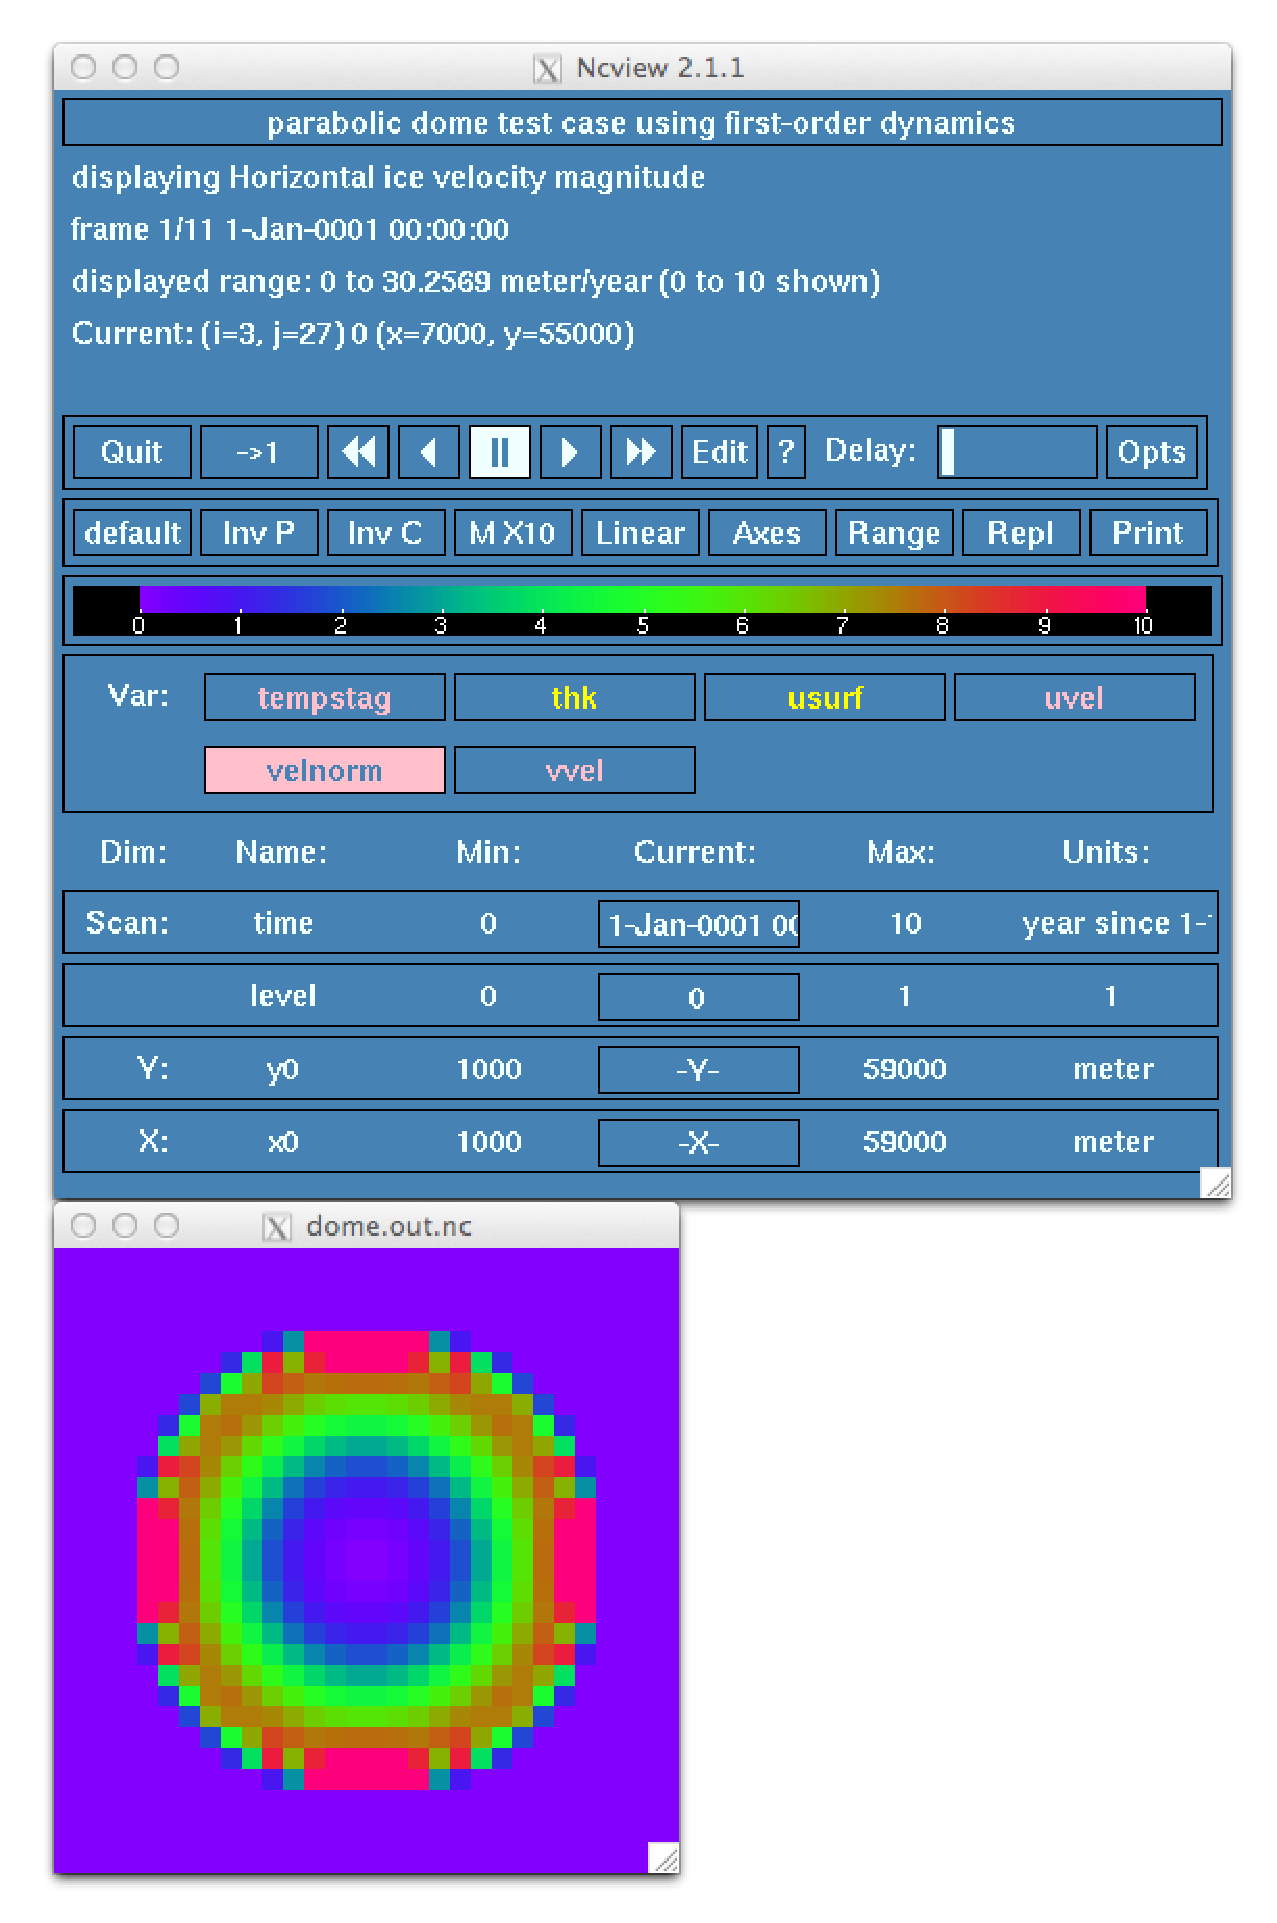
\includegraphics[width=7.0cm]{\dir/dome-output.eps}
	\caption{Dome velnorm (i.e., the ice speed in m/yr) field at time 0 using default \texttt{dome.config} settings. This figure is a screenshot of ncview.}
	\label{fig:domeresults}
\end{figure}
\FloatBarrier

% =====================================
\subsection{ISMIP-HOM}
% =====================================
The Ice Sheet Model Intercomparison Project for Higher-Order Models (ISMIP-HOM)
prescribes a set of experiments meant to test the implementation of higher-order physics.  
For more information, see \href{http://homepages.ulb.ac.be/~fpattyn/ismip/}{here}
\footnote{http://homepages.ulb.ac.be/~fpattyn/ismip/} and the ISMIP-HOM description paper by \citet{Pattyn2008}.

The python scripts provided (runISMIPHOM.py and plotISMIPHOM.py, refered to in the following as the ISMIP-HOM 
scripts) were created to run experiments A through F using CISM and compare the results with results from other models. 

Note: The \texttt{README} file describes many additional details about running and analyzing the
test case that are not described here.

\subsubsection{Provided Files}

\begin{itemize}
	\item README \\
		Information about the test case, including technical details about running it.
	\item ishom.config \\
		A default configuration file used as a template for generating the .config file for each test.
    		If you wish to run the tests with different solver settings, for example, you should edit this file.
	\item runISMIPHOM.py \\
		The script used for running any/all of the ISMIP-HOM experiments.  
    		Invoke with `- - help' to see the many command line options for controlling execution.
  \item plotISMIPHOM.py \\
		The script used for analyzing/plotting any/all of the ISMIP-HOM experiments.  
    		Invoke with `- - help' to see the many command line options for controlling execution.
\end{itemize}

\subsubsection{Running the test}
One script sets up the initial condition and runs the model:

\texttt{./runISMIPHOM.py}

and another is used to analyze the results:

\texttt{./plotISMIPHOM.py}

\subsubsection{Results}
The \texttt{plotISMIPHOM.py} script will plot results relative to other models.
None of the ISMIP-HOM tests have a useful analytic solution, so these tests are
used as community benchmarks rather than actual model verification tests.
Therefore, the \citet{Pattyn2008} paper is useful for intepreting model results.
An example output plot is shown in Figure \ref{fig:ismiphom-results}.

\begin{figure}[H!]
	\centering
	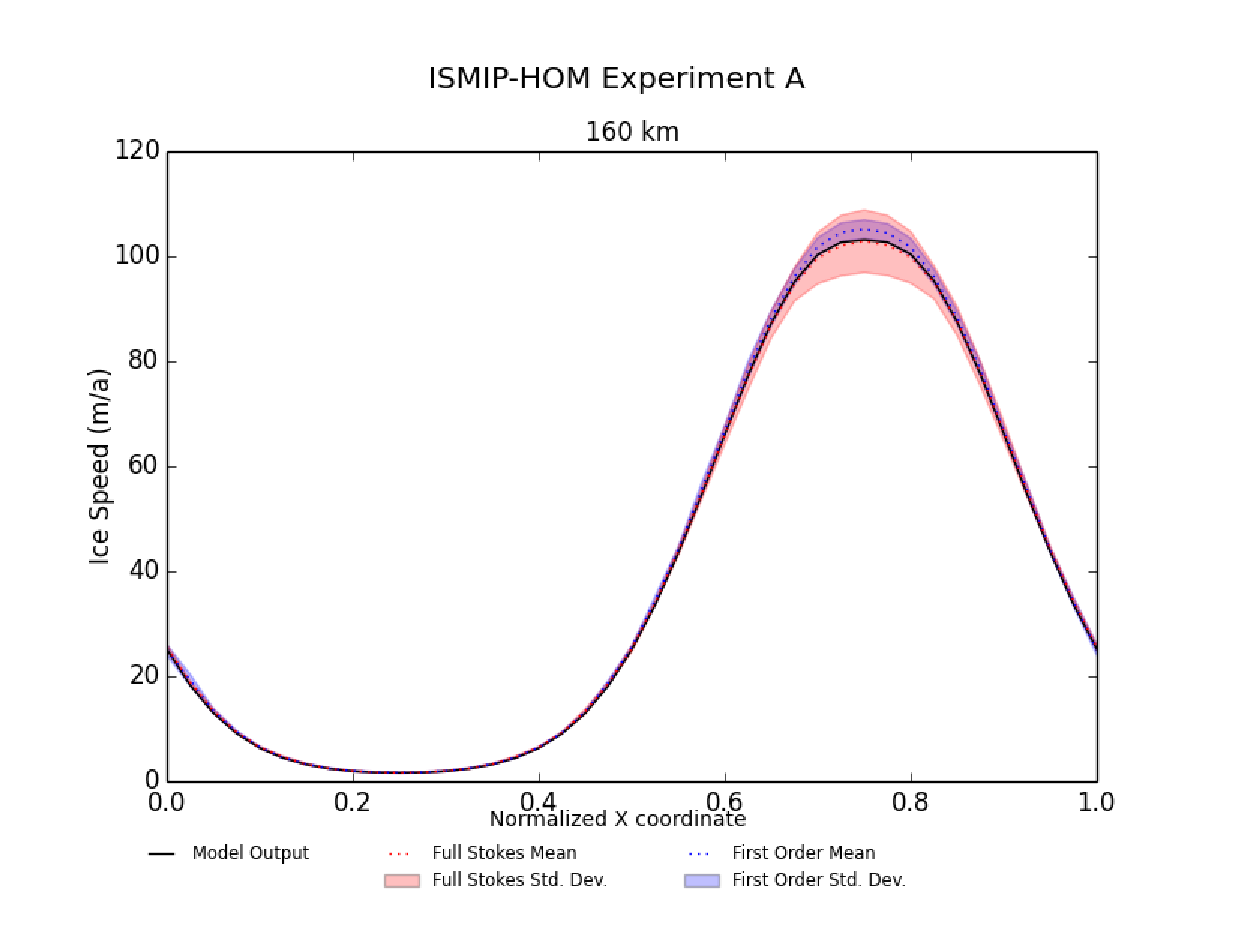
\includegraphics[width=10.0cm]{\dir/ISMIP-HOM-A-cis1.eps}
	\caption{An example of the ISMIP-HOM test case output for test A at size L=160 km. 
CISM output is shown with black line and the range of output from other models is shown by colored bars. 
This figure was generated with \texttt{./plotISMIPHOM.py -e a -s 160} after running the test with \texttt{./runISMIPHOM.py -e a -s 160}.
Additional options (e.g., running and plotting for multiple tests simultaneously) are described in the \texttt{README} and by invoking the
`- - help' option at the command line.}
	\label{fig:ismiphom-results}
\end{figure}
\FloatBarrier

% =====================================
\subsection{Stream}
% =====================================

This test case simulates flow over an idealized ice stream underlain by a subglacial till with a known and specified
yield stress distribution (also, see discussion in Section \ref{sc:higher-order-bcs}). For the two distributions available in this test case, 
analytical solutions are available from \citet{Raymond2000} and \citet{Schoof2006}. 

For the Raymond test case, the yield stress within the ice stream is given a uniform value below the driving stress, and outside of the
ice stream it is given a uniform value much higher than the driving stress (i.e., the yield stress distribution is approximated by a
``step" function). For the Schoof test case, the till yield stress across the ice stream is given by a continuously varying function.

In both cases, the basal properties vary in the across-flow direction only and are symmetric about the ice stream centerline.
As a result, the velocity solutions are also uniform along flow and symmetric about the centerline.

\subsubsection{Provided Files}

\begin{itemize}
	\item README \\
		Information about the test case, including technical details about running it.
	\item runStream.py \\
		The script to setup and run the test test.
	\item stream.config.in \\
  The default configuration settings for running CISM with the test case. Note that this
  file is parsed by the runStream.py script. Most of the relevant options that might be changed
  for this test case (e.g., grid spacing) can be done so from the command line, without having to
  edit the .config files (use \texttt{./runStream.py --help} to obtain a description of available options.
  The choice of test case - using the Raymond or Schoof yield stress distribution -  can be toggled 
  by editing line 15 of the runStream.py script.
\end{itemize}

\subsubsection{Running the test}
One script sets up the initial condition and runs the model:

\texttt{./runStream.py}

and another is used to analyze the results:

\texttt{./plotStream.py}

\subsubsection{Results}
The \texttt{plotStream.py} script will plot model output relative to the analytical solutions
given in \citet{Raymond2000} and \citet{Schoof2006}. The choice of analytical solution to compare
to is decided on automatically, based on what value is currently active in the runStream.py script. 
Example output for both test cases is shown in Figure \ref{fig:stream-results}.
	
\begin{figure}[H!]
  \begin{center}
	\includegraphics[width=10.0cm]{\dir/stream_raymond.eps}
	\includegraphics[width=10.0cm]{\dir/stream_schoof.eps}
  \end{center}
  \caption{Comparison between CISM model output (black) and analytic solution (red) for the Raymond (top) and Schoof (bottom) stream test cases. This figure was generated with \texttt{./plotStream.py} after running the test with \texttt{./runStream.py}.
Additional runtime options are described in the \texttt{README} and by invoking the `- - help' option at the command line.}
  \label{fig:stream-results}
\end{figure} 

% =====================================
\subsection{Confined Shelf}
% =====================================
This test setup is from tests 3 and 4 from the idealized (i.e. not Ross) EISMINT-shelf test 
cases.  It simulates the flow within an idealized, 500 m thick ice shelf in a 
confined, rectangular embayment.  Grounded ice is not explicitly modeled but included in the 
model setup as Dirichlet boundary conditions for velocity along the ice shelf edges.
More detailed information on this test case can be found 
\href{http://homepages.vub.ac.be/~phuybrec/eismint/iceshelf.html}{here}
\footnote{http://homepages.vub.ac.be/~phuybrec/eismint/iceshelf.html} in the 
``shelf-descr.pdf" document.

Note that the Confined Shelf and Circular Shelf experiments are both in the 
\texttt{tests/higher-order/shelf} directory and share some files.

\subsubsection{Provided Files}

\begin{itemize}
	\item README \\
		Information about the test case, including technical details about running it.
	\item confined-shelf.py \\
		The script to setup and run the test test.
	\item confined-shelf.config \\
  The default configuration settings for running CISM with the test case.
\end{itemize}

\subsubsection{Running the test}
One script sets up the initial condition and runs the model:

\texttt{./confined-shelf.py}

\subsubsection{Results}
There is not a script for analyzing the results.  See the URL above for information 
about assessing the model output.
You can manually inspect the results using a tool such as \texttt{ncview}.
An example is shown in Figure \ref{fig:confinedshelf-results}.

\begin{figure}[H!]
	\centering
	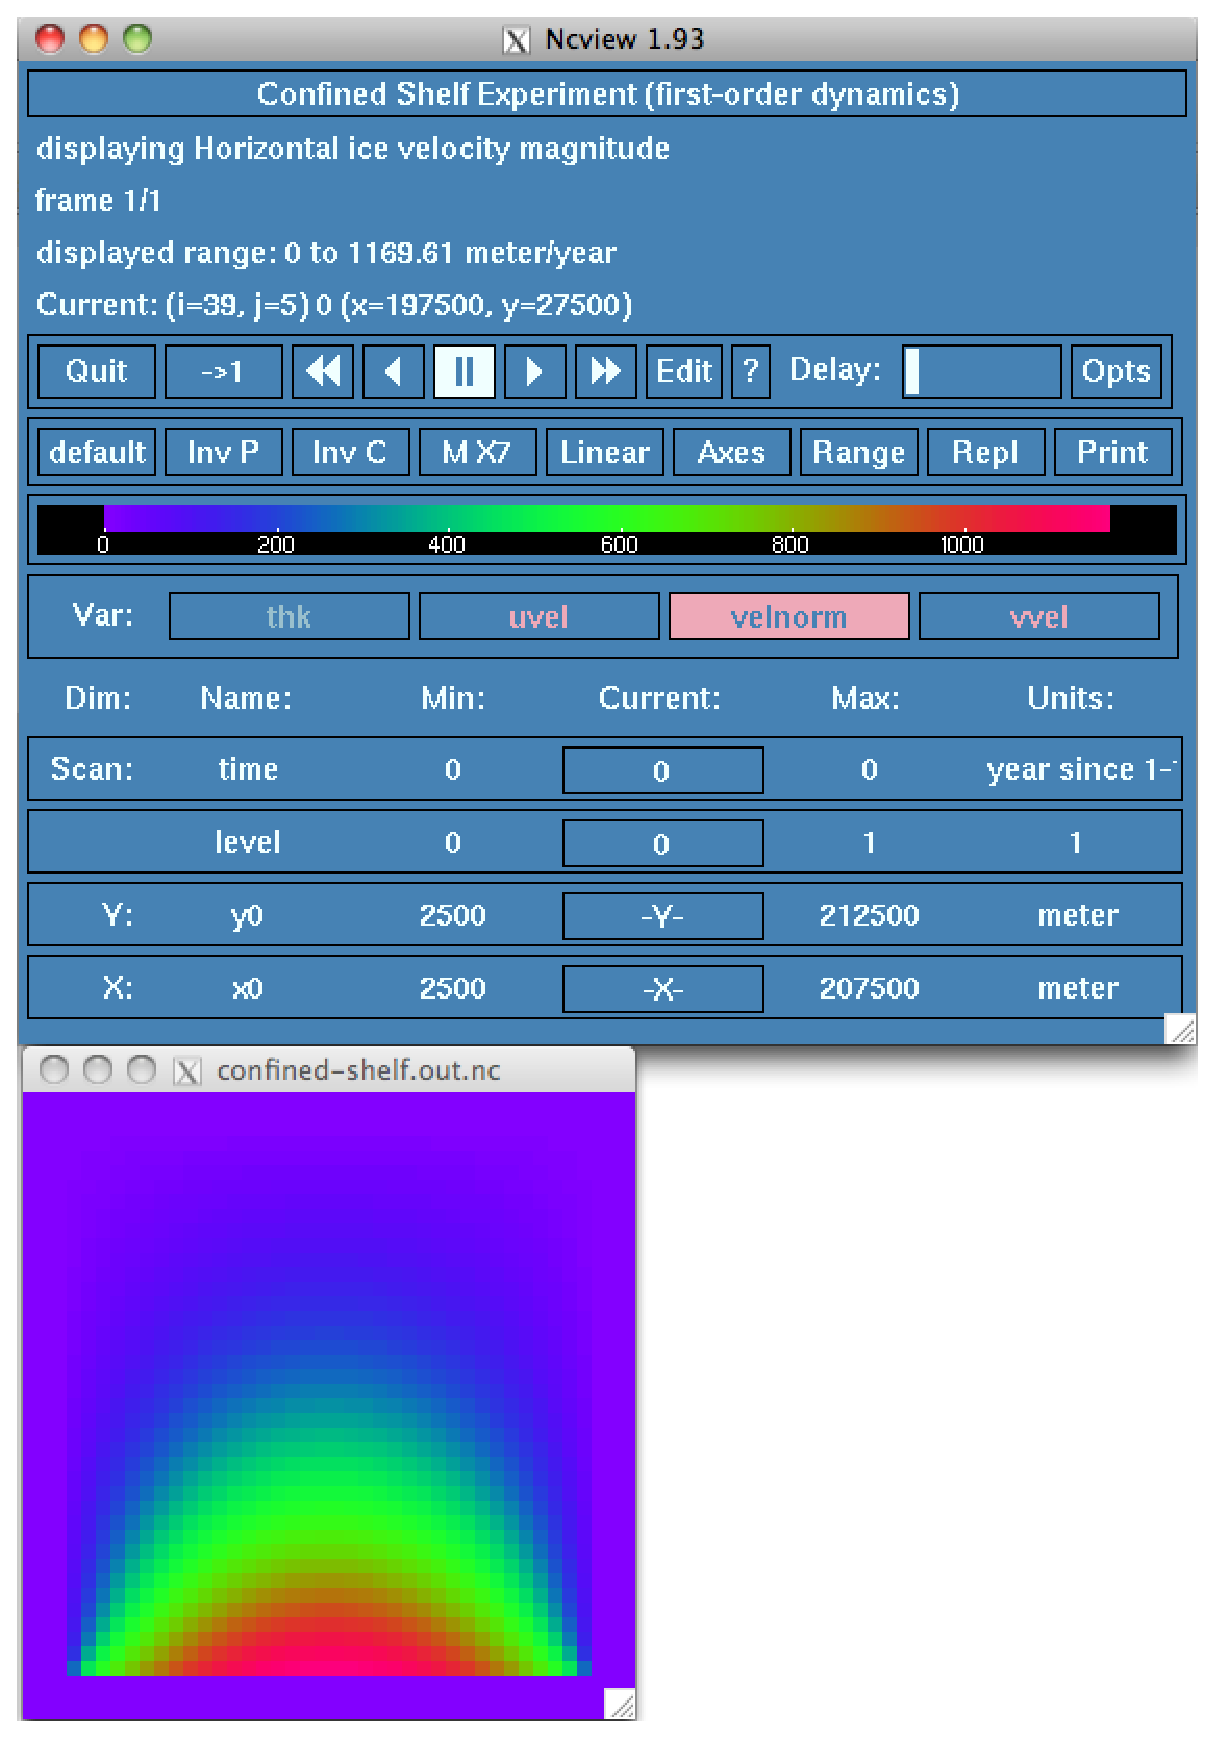
\includegraphics[width=8.0cm]{\dir/confinedshelf-output.eps}
	\caption{Confined shelf velnorm field using default \texttt{confined-shelf.config} settings. This figure is a screenshot of ncview.}
	\label{fig:confinedshelf-results}
\end{figure}
\FloatBarrier

% =====================================
\subsection{Circular Shelf}
% =====================================
This test is a variant on the confined shelf test case discussed above. It simulates the flow within a circular ice shelf with a uniform thickness
of 1000 m, which is grounded at a single grid point at its center. This test case confirms a working ``floating ice" boundary condition implementation
in two dimensions (i.e, in map plane view) and also confirms radial symmetry. 

Note that the Confined Shelf and Circular Shelf experiments are both in the 
\texttt{tests/higher-order/shelf} directory and share some files.

\subsubsection{Provided Files}

\begin{itemize}
	\item README \\
		Information about the test case, including technical details about running it.
	\item circular-shelf.py \\
		The script to setup and run the test test.
	\item circular-shelf.config \\
  The default configuration settings for running CISM with the test case.
\end{itemize}

\subsubsection{Running the test}
One script sets up the initial condition and runs the model:

\texttt{./circular-shelf.py}

\subsubsection{Results}
There is not a script for analyzing the results.
You can manually inspect the results using a tool such as \texttt{ncview}.
An example is shown in Figure \ref{fig:circularshelf-results}.

\begin{figure}[H!]
	\centering
	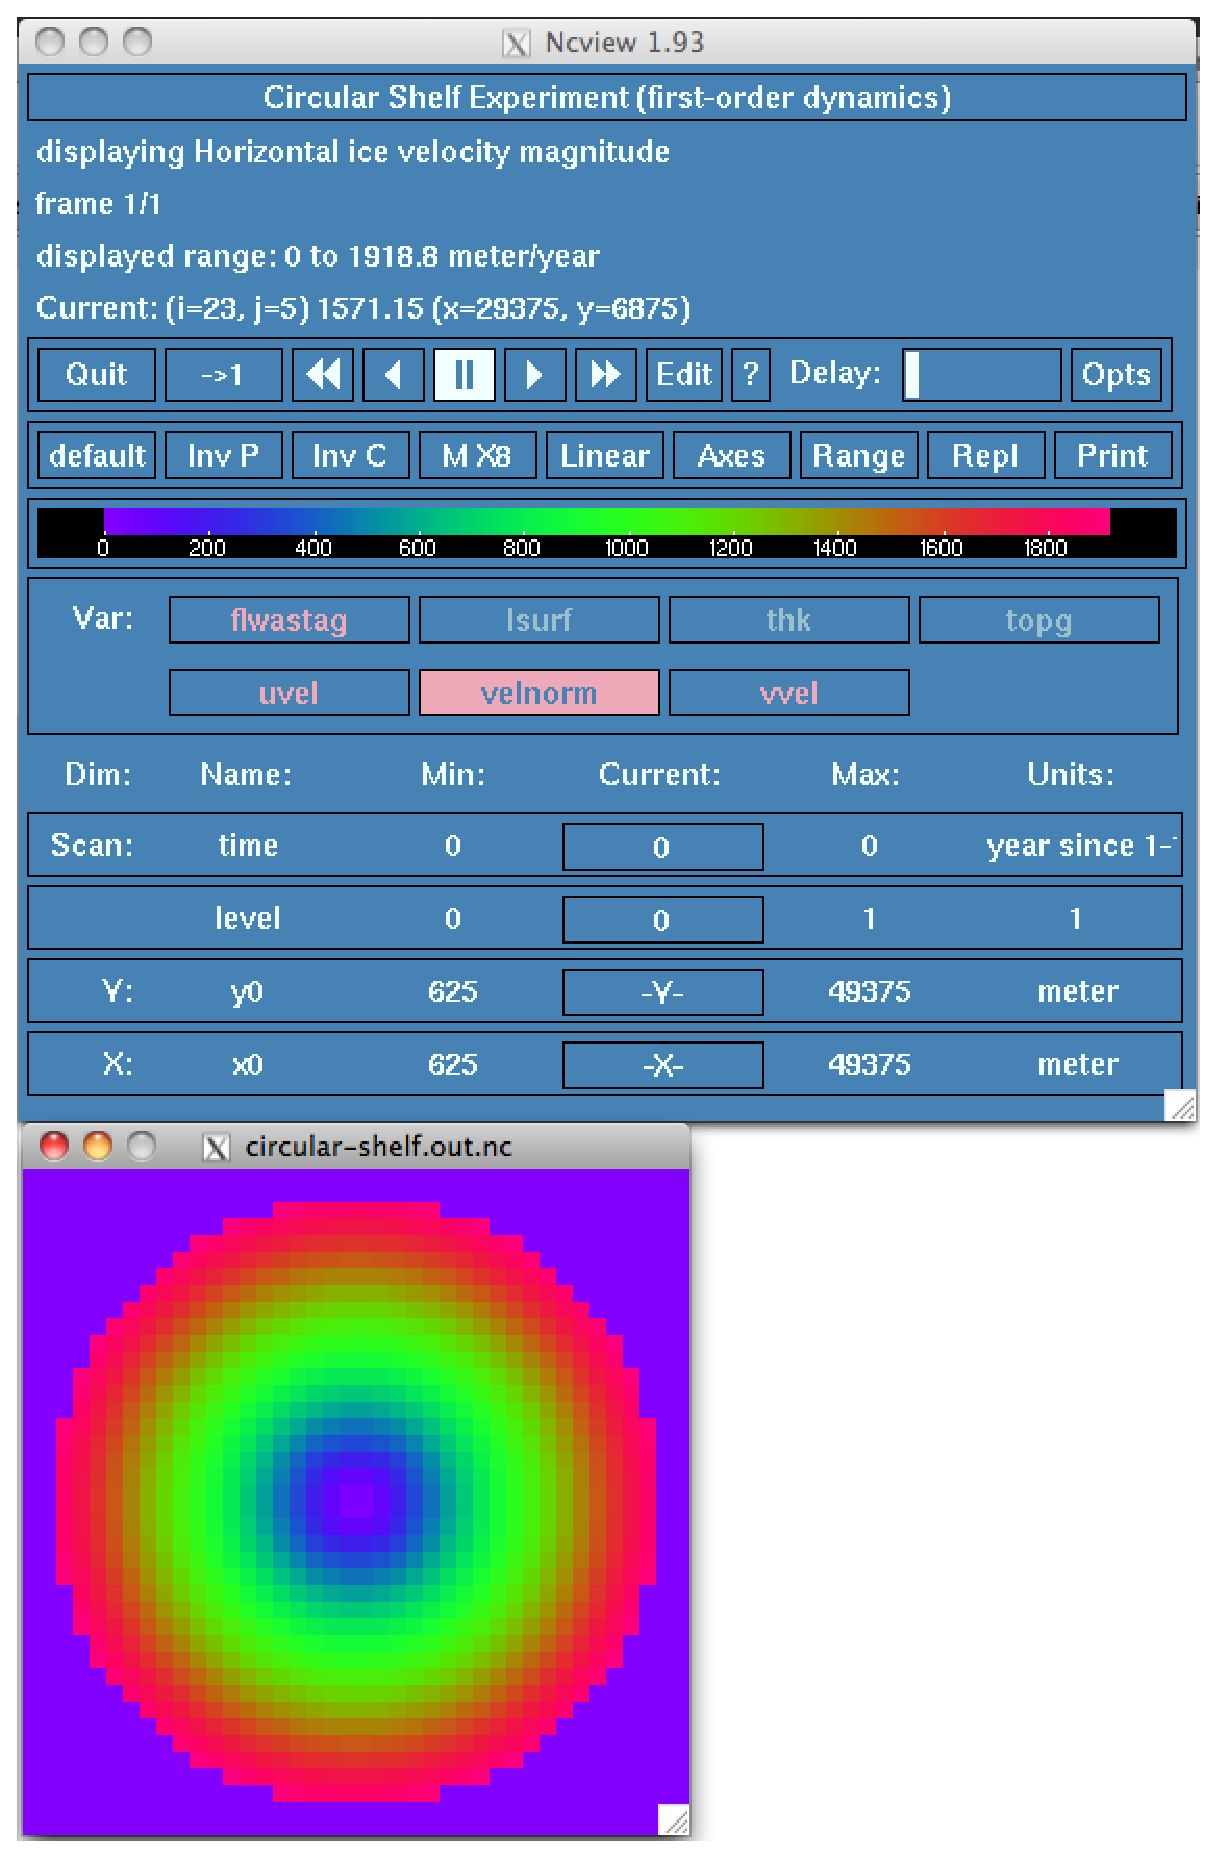
\includegraphics[width=8.0cm]{\dir/circularshelf-output.eps}
	\caption{Circular shelf velnorm field using default \texttt{circular-shelf.config} settings. This figure is a screenshot of ncview.}
	\label{fig:circularshelf-results}
\end{figure}
\FloatBarrier

% =====================================
\subsection{Ross Ice Shelf}
% =====================================
This experiment was designed to simulate the flow of the Ross Ice Shelf of Antarctica under idealized conditions (e.g., constant and uniform
flow-law rate factor). For more information about the experiment and its results see 
\href{http://homepages.vub.ac.be/~phuybrec/eismint/iceshelf.html}{here}\footnote{http://homepages.vub.ac.be/~phuybrec/eismint/iceshelf.html}. 
Also, see \citet{MacAyeal:1996vn} for a discussion of the official model intercomparison results.

This experiment will typically take about 10 minutes to run on a single processor.

\subsubsection{Provided Files}

\begin{itemize}
	\item README \\
		Information about the test case, including technical details about running it.
	\item runRoss.py \\
		The script to setup and run the test test.
	\item ross.config \\
  The default configuration settings for running CISM with the test case.
	\item plotRoss.py \\
		The script to plot the test results.
\end{itemize}

\subsubsection{Running the test}
One script sets up the initial condition and runs the model:

\texttt{./runRoss.py}

and another can be used to visualize the results:

\texttt{./plotRoss.py}

\subsubsection{Results}
The \texttt{plotRoss.py} script will generate a figure of the velocity field
calculated for the Ross Ice Shelf.  The results should look very similar to Figures \ref{fig:rossresults1} and \ref{fig:rossresults2}. You can
compare these with similar figures in the paper by \citet{MacAyeal:1996vn}.

\begin{figure}[H!]
	\centering
	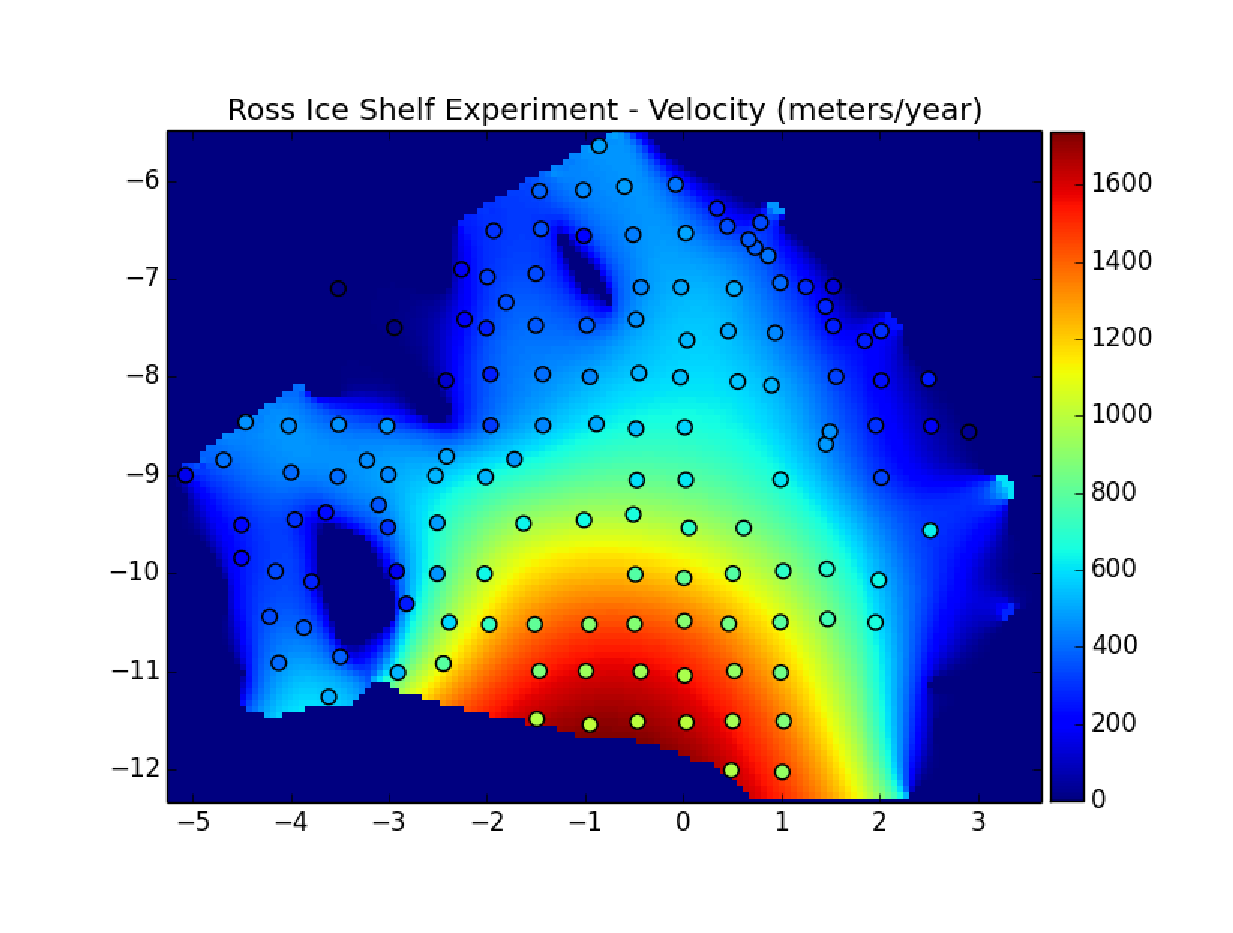
\includegraphics[width=10.0cm]{\dir/RossModelVelField.eps}
	\caption{Ross Ice Shelf velocity field calculated by CISM. This figure is generated by \texttt{plotRoss.py}.}
	\label{fig:rossresults1}
\end{figure}
%\FloatBarrier

\begin{figure}[H!]
	\centering
	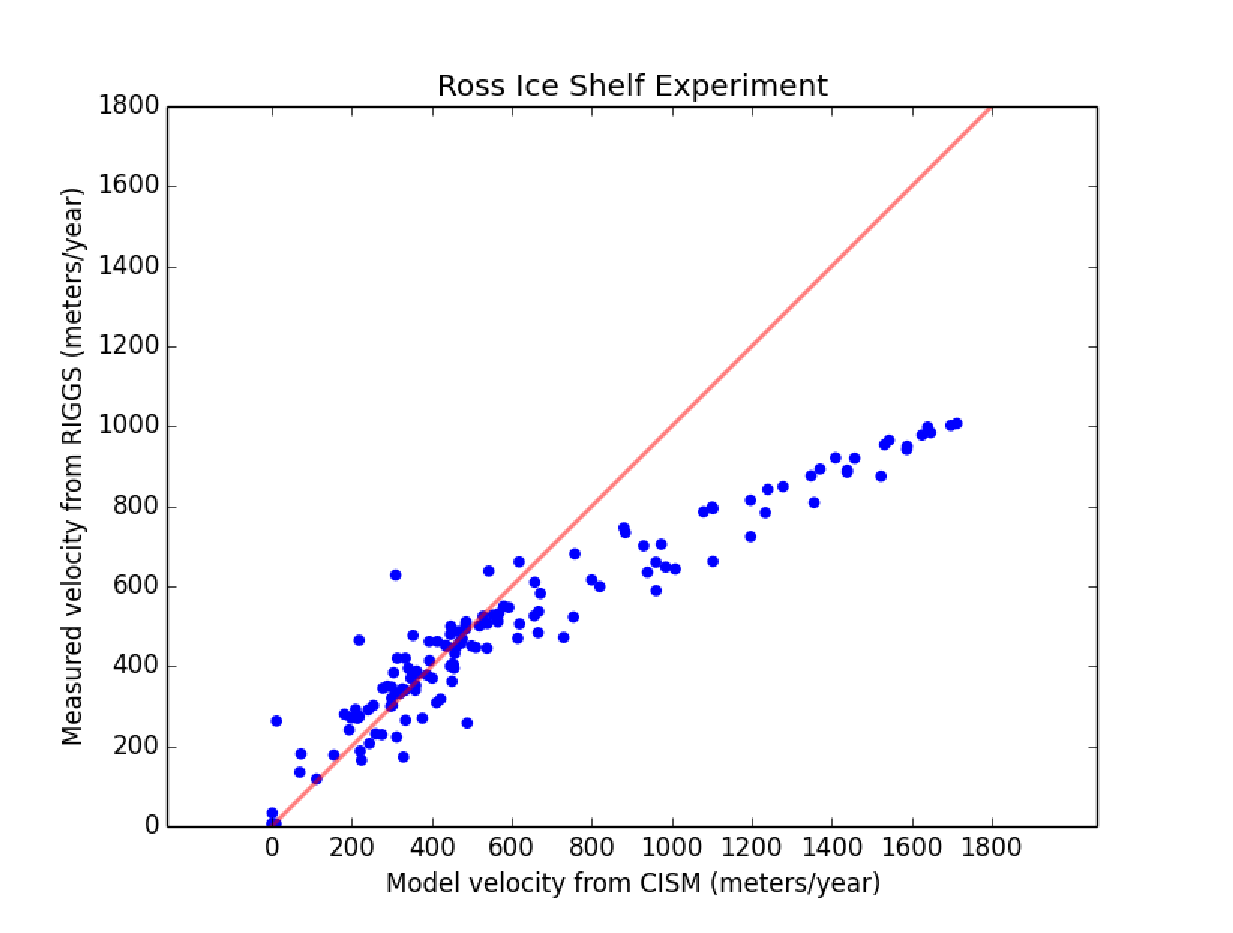
\includegraphics[width=10.0cm]{\dir/RossModelvsObs.eps}
	\caption{CISM-modeled Ross Ice Shelf speeds vs. those from observations. This figure is generated by \texttt{plotRoss.py}.}
	\label{fig:rossresults2}
\end{figure}
\FloatBarrier


% =====================================
\subsection{Other Tests}
% =====================================
Additional higher-order tests that are still in development (e.g., ``slab" and ``stream") are also included in the \texttt{./tests/higher-order/}
directory. Instructions for how to run these tests are included in each directory. However, since these tests have not yet been validated yet, 
they are for use at your own risk.




